\chapter{Discussion}
\label{ch:Discussion}
The chapter on Discussion covers the entire work and, in particular, the results achieved in \autoref{ch:ResultsAnalysis}. In the following sections, the results will be interpreted, the objectives of the thesis will be reviewed, and recommendations for future research in teledermatology image quality assessment will be provided. \par
\section{Interpretation of Results}
\label{sec:InterpretationResults}
The differences in model performance shown in \autoref{fig:ModelSRCC} reveal that both classifiers (XGB Classifier and MLP Classifier) were not as effective as the regressors (XGB Regressor and MLP Regressor). This is likely because the task involves predicting continuous severity scores, which are more suited to regression models. Classifiers categorize the severity into fixed levels, which can lead to less precise predictions.\par \todo{check this paragraph}
\vspace{\baselineskip}
\noindent
The experiments demonstrated that the cross-dataset evaluation showed good generalization. The models performed well not only on the datasets they were trained on but also on previously unseen datasets. This indicates that the models, especially the MLP Regressor, can generalize well to different data distributions and are robust.\par
\subsection{Analysis of Individual Distortion Criteria}
\label{subsec:AnalysisDistortionCriteria}
When we analyze the metrics in \autoref{table:performance_metrics} alongside the confusion plots in \autoref{fig:confusion_matrices}, it becomes clear that the criteria for focus, color calibration, and resolution are captured very well by the model. Although there are some fluctuations between the predicted severity and the actual severity, these deviations are typically only by one severity level. This minor difference suggests that the model is making reasonably accurate predictions. This high level of accuracy can be explained by the design of the ARNIQA backbone. When training ARNIQA to extract features, their goal was to assess general image quality, and they focused also on distortions related to focus and color calibration. Since I am using their backbone to extract features, the model performs better in these criteria.\par
\vspace{\baselineskip}
\noindent
On the other hand, lighting was also one of the distortions that ARNIQA focused on, but this criterion performed only moderately well. This can be reasonably explained by the fact that the lighting criterion includes two opposite types of distortions: brightening and darkening. If the majority of the training images were brightened and the validation set included darkened images, this could negatively impact performance. That is why the model struggles to accurately predict the lighting severity due to these opposing distortion types.\par
\vspace{\baselineskip}
\noindent
For the background criterion, it is clear from the confusion plot that there are rarely predictions on the higher severity levels. This is because, in the distortion pipeline, if the background proportion is less than 10\% relative to the skin, no color blocks are added, resulting in a 0 value for background distortion. This indicates that many images were given a 0 value for background distortion. Additionally, when looking at the radar chart of the combined synthetically distorted images in \autoref{fig:comb_synthetic}, the median value for background distortion is lower than that of other criteria, indicating fewer strong severity values. \par
\begin{comment}
    This hypothesis that including more images with significant background presence can improve the model’s performance is supported when examining the radar charts of filtered SCIN and filtered Fitzpatrick images in \autoref{fig:SF} and \autoref{fig:FF}. The median severity for SCIN images is lower compared to the Fitzpatrick dataset. Moreover, the predictions for individual datasets also show differences. For example, \autoref{table:background_metrics} compares the metrics for background distortion between SCIN and Fitzpatrick using an MLP regressor. This table shows that the regressor trained on synthetically distorted SCIN images performs better on background. This further indicates that enhancing the training dataset with more background inclusive images could address this issue effectively.\par
\end{comment}
\vspace{\baselineskip}
\noindent
The confusion plot also shows that the orientation criterion is generally uncertain in its predictions, tending to cluster around the middle severity levels. This might be due to the various perspective changes (top, bottom, right, left) applied during training. As a result, the model detects that there is some perspective distortion but cannot precisely determine the direction or severity, leading to predictions that hover around the middle severity levels.\par
\vspace{\baselineskip}
\noindent
Field of view distortion was the most experimental criterion. In teledermatology, it is crucial to have the lesion or area of interest centered in the image. However, in general photography, the subject is often placed off-center to create a more aesthetically pleasing composition. This is why ARNIQA, trained for general image quality assessment, might have difficulties with field of view distortions specific to teledermatology. This was confirmed by comparing the performance metrics between SCIN and Fitzpatrick images, where Fitzpatrick images performed better in field of view distortion, likely due to having less background (see \autoref{table:fov_metrics} and compare \autoref{fig:SF} with \autoref{fig:FF}). \par
 \begin{table}[ht]
    \centering
    \begin{tabular}{|l|c|c|c|c|}
        \hline
        \textbf{Dataset} & \textbf{MAE} & \textbf{R\textsuperscript{2}} & \textbf{SRCC} & \textbf{Cohen's Kappa} \\
        \hline
        SCIN (synthetically distorted) & 1.20 & 0.05 & 0.23 & 0.08 \\
        F17K (synthetically distorted) & 0.63 & 0.50 & 0.72 & 0.71 \\
        \hline
    \end{tabular}
    \caption{Performance metrics for field of view distortion using an MLP regressor on synthetically distorted SCIN and F17K images. F17K refers to the Fitzpatrick17k images.}
    \label{table:fov_metrics}
\end{table}
% Background     |   1.1246   |   0.1010   |   0.3377   |     0.2654
% Field of view    |   1.2020   |   0.0513   |   0.2293   |     0.0845 

% Background     |   1.1439   |   0.1742   |   0.4573   |     0.3024 
% Field of view    |   0.6288   |   0.5081   |   0.7175   |     0.7064
\noindent
These observations highlight the strengths of using a combined dataset. By integrating diverse images from different sources, the model benefits from a wider variety of distortions and scenarios, enhancing its ability to generalize and perform well across different conditions. \par

\subsection{Overall Model Performance on Test Sets}
\label{subsec:OverallModelPerformance}
\subsubsection{Synthetic Distorted Images}
\label{subsubsec:SyntheticDistortedImages}
The model’s performance on the 70 synthetic distorted test images aligns well with the validation split and the cross-dataset evaluation, as shown in \autoref{fig:synthetic}. In this figure, I randomly selected some images, and the four-column layout presents the original image, the distorted image, the actual labels, and the model’s predictions.\par
\vspace{\baselineskip}
\noindent
First, let’s discuss background distortion. The actual severity matches closely with the predictions for most images. To further improve the model’s performance, an experiment I didn’t have time to conduct would involve applying color blocks randomly on the whole image without any skin segmentation. This approach, though unconventional for teledermatology images, could test the model’s robustness by introducing random artifacts. The second and fourth images in \autoref{fig:synthetic} suggest this method could work effectively.\par
\vspace{\baselineskip}
\noindent
One noticeable issue is the field of view distortion, where the predictions are not accurate. Despite background, lighting, and orientation distortions not being well-represented in the confusion plot in \autoref{fig:confusion_matrices}, they appear to be quite accurate in the synthetic test set images shown. This suggests that while the confusion plot highlights general trends, individual image predictions can vary. \par
\vspace{\baselineskip}
\noindent
One important factor to consider is the distribution of distortion severity levels. The distortion pipeline selects ranges randomly. To improve this, I experimented with choosing distortion ranges according to a Gaussian distribution centered at 0 severity with a standard deviation of 2.5. This approach might include more distortions with lower severity, which are more common in teledermatology images. For instance, heavily brightened images, as seen in the last synthetic distorted image, may not occur frequently in real-world scenarios. Training the model on more common distortions could enhance its performance. This experiment was initiated, but no evaluation could be conducted due to time constraints. \par

\subsubsection{Authentic Test Images}
\label{subsubsec:AuthenticTestImages}
For the 200 authentic test images, random samples are shown where I labeled the images. At first look, the predictions do not match my labels well. This difference could be due to several factors. Firstly, I labeled the images primarily by focusing on the skin lesion, often ignoring the background, which might not align with the model’s overall assessment. Labeling 1,400 instances (200 images, 7 criteria each) likely introduced some human error. \par
\vspace{\baselineskip}
\noindent
Also, images with multiple distortions complicate the assessment of individual criteria. For instance, a heavily darkened image might hide other distortions like focus, resolution, and color calibration, making it difficult to evaluate accurately. Additionally, labeling lesions or marks on darker skin tones presented challenges, which might have affected the labeling accuracy. This highlights the broader issue of skin tone diversity in medical imaging, an important factor that was not within the scope of this thesis but is worth mentioning for future research.\par
\vspace{\baselineskip}
\noindent
Despite these challenges, if we take out the field of view distortion, the model’s predictions are quite accurate. This distortion significantly affects the radar charts. I chose not to label the images again to avoid “leaking information” from the test set into the training process, keeping the evaluation fair and accurate. \par

\subsection{Comparison with ARNIQA Predictions}
\label{subsec:ComparisonARNIQA}
The first thing to note is that ARNIQA predicts image quality scores ranging from 0 to 1, where higher values indicate better image quality. In contrast, my model predicts distortion severity scores, also ranging from 0 to 1, but where higher values indicate worse image quality. My model also evaluates seven different criteria, and to make a direct comparison with ARNIQA’s single quality score, I took the median of all distortion scores. This provides a single, balanced score that represents the overall quality of the image by aggregating the severity of distortions across all criteria. Additionally, the scores from ARNIQA had to be inverted for comparison. ARNIQA also provides six different regressors for image evaluation, and for this analysis, I used the default regressor, which was trained on the KADID10K dataset. \par
\vspace{\baselineskip}
\noindent
\autoref{fig:T2A} and \autoref{fig:T7A} show the differences in predictions. ARNIQA tends to predict that all images have very low quality, while my model’s predictions align more closely with both the self-labeled values and the synthetically generated values. This suggests that while ARNIQA is highly sensitive to distortions, it may not be as finely tuned to the specific context of teledermatology as my model. \par
\vspace{\baselineskip}
\noindent
To further validate ARNIQA’s ability to differentiate image quality, I compared its predictions on 70 filtered good quality images with those on synthetically distorted images. As shown in \autoref{fig:T7A2}, ARNIQA can indeed distinguish between good and bad quality images, confirming its general effectiveness. However, my approach of using synthetically distorted images appears to improve performance in teledermatology-specific tasks, as my model’s predictions align better with the expected outcomes in this domain. \par
\begin{figure}[ht]
    \centering
    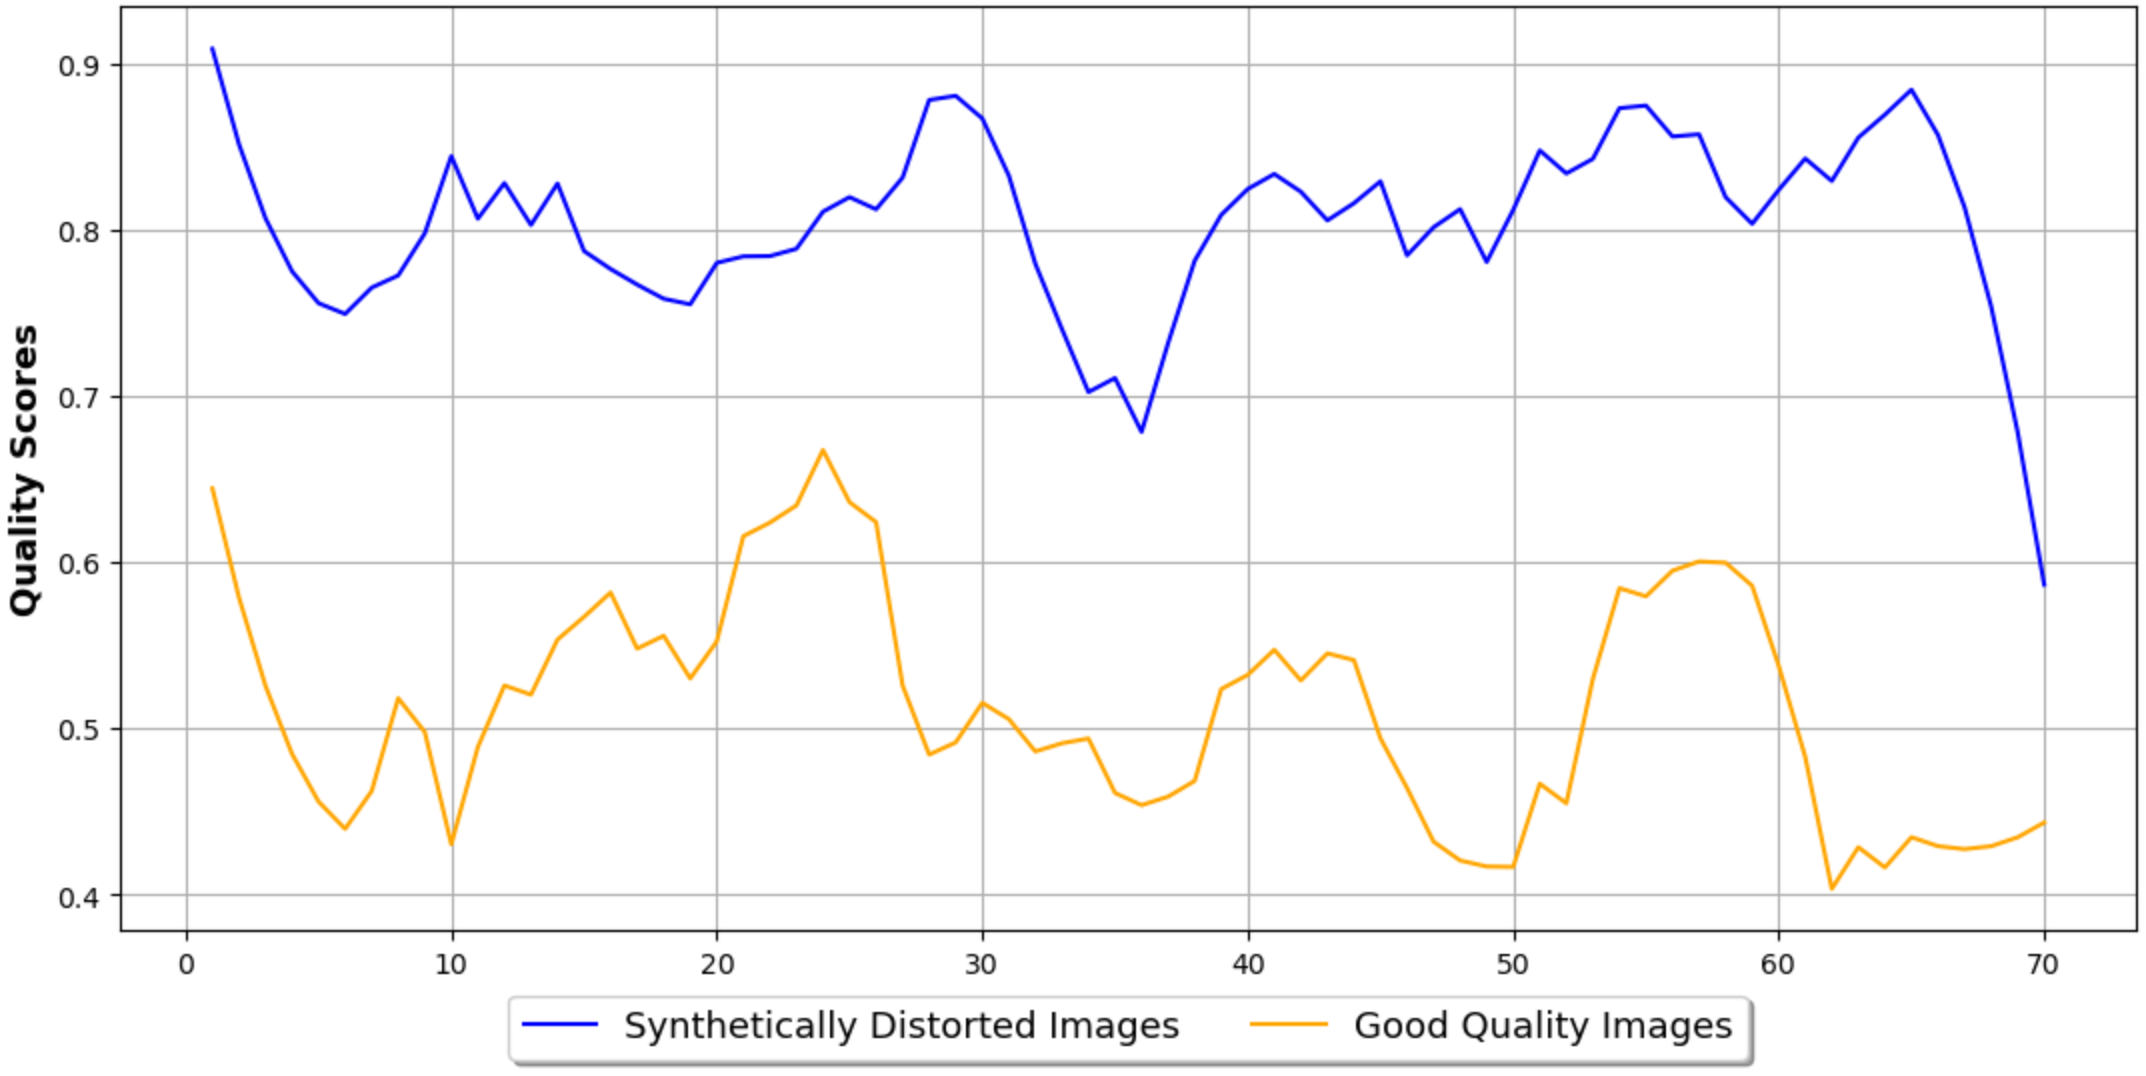
\includegraphics[keepaspectratio,width=15cm]{img/hept/test_70_arniqa2.png}
    \caption{Comparison of ARNIQA’s quality scores for 70 synthetically distorted images (blue) and 70 good quality images (orange). The scores range from 0 to 1, where higher values indicate better image quality.}
    \label{fig:T7A2}
\end{figure}
\noindent
These comparisons highlight the strengths of a domain-specific approach and suggest that while general image quality assessment models like ARNIQA are useful, customized models tailored to specific applications can offer significant improvements. My approach of synthetically distorting images and training the model specifically for teledermatology not only aligns better with the expected outcomes but also enhances the model’s robustness and accuracy in this specific field. \par
\section{Key Model Assumptions and Their Implications}
\label{sec:KeyModelAssumptions}
The models assume that the features extracted by ARNIQA’s backbone are comprehensive enough to capture the key distortions in teledermatology images. This assumption holds true for lighting, focus, color calibration, and resolution, covering 4 out of the 7 criteria. The remaining criteria: background, orientation, and field of view need further experimentation and fine-tuning. While the current performance indicates some level of effectiveness, more targeted data collection and model adjustments are necessary to fully validate these assumptions.\par
\vspace{\baselineskip}
\noindent
If the assumption that ARNIQA’s backbone can capture all key distortions is not entirely correct, it would mean that the model might not perform well in real-world scenarios where these distortions are prevalent. To ensure these assumptions are valid, additional experiments with varied datasets and real-world images should be conducted. By expanding the variety of images used in training, particularly those with significant background presence, the model can be better equipped to handle real-world distortions. This is crucial for improving the model’s robustness and generalizability.\par
\vspace{\baselineskip}
\noindent
While the backbone has proven effective for certain distortions, the uncertainties with background and orientation distortions highlight the need for further refinement. Addressing these uncertainties through targeted data collection and further model tuning can enhance the overall performance and reliability of the image quality assessment in teledermatology. Overall, the ARNIQA backbone shows great potential for teledermatology applications, but continuous improvement and validation are essential to achieve the best possible performance.\par

\section{Reviewing the Objectives of the Thesis}
\label{sec:ReviewingObjectives}
At the beginning of this thesis, the specific objectives were detailed:

\begin{itemize}
    \item An extensive review of the literature on image quality assessment (IQA) methods, focusing on their application in teledermatology.
    \item Identifying and selecting image quality metrics that are most suitable for assessing the quality of dermatological images.
    \item Evaluate the performance of selected image quality metrics on dermatological datasets to determine their effectiveness in assessing image quality.
    \item Develop a reproducible repository of image quality assessment tools and methodologies for teledermatology applications.
\end{itemize}
\noindent
The first objective involved carrying out an in-depth review of the literature on image quality assessment methods and their application in teledermatology. This took a lot of time but was very important for the rest of the work. Through this review, key concepts such as IQA, teledermatology, ARNIQA, and related works were explored and documented. \par
\vspace{\baselineskip}
\noindent
The second objective was achieved during the literature review process. In this phase, the seven quality criteria from ISIC were identified and chosen as the best metrics for assessing the quality of dermatological images. This selection was critical for the next steps. \par
\vspace{\baselineskip}
\noindent
For the third objective, the performance of the selected image quality metrics was evaluated on dermatological datasets. These evaluations were thorough, involving tests on independent images not included in the model training. The datasets included both synthetically distorted images and images with authentic distortions, ensuring a complete assessment of how well the metrics worked. \par
\vspace{\baselineskip}
\noindent
The final objective was to develop a reproducible repository of image quality assessment tools and methods for teledermatology applications. This was successfully accomplished, making it possible for further experiments and research to build on this thesis. The repository provides a solid framework for future work in this field, ensuring that the methods and tools developed here can be effectively used and expanded upon. \par
\section{Comparison with Related Work}
\label{sec:ComparisonRelatedWork}

\section{Reflection}
\label{sec:Reflection}
\begin{comment}
    great now on section reflexion.
in all the the work showed me that assessimg image quality in context of teledermatology is possible with my approach. this can be further experimented with and used as reference. or used in dermatolgoy images, where lighting, focus, color calibration and resolution are mainly present than background, orientation and field of view are less the case as they can be taken with dermascope or in a controlled setting. At the research  and development their were difficult and easier phase. The begining was in comparison difficult, gathering domain knowledge, understanding key concepts, not going to in depth on each topic and synthesizing information and having still a broad view on the objectives were difficult. luckily these hurdles could be overcome. synthetically creating distortions and using the severity ranges as values was very fastinating as this tackles the problem of having not many image data and more very rarely having annotated image datasets.the most time consuming or lets say gruiling and unwanted part was filtering good quality images and also labeling the test set.  the most difficult phase was experimenting. as i tried to understand every detail of ARNIQA first and on that backtracking on how the images need to be so that the features can be extracted. also finding the some what correct representation of the images in the different severity ranges. As it turns out finding the correct way to represent each distortion for the model to understand is very important. their also plays the role that the images used need to be good quality also. The goal of the experimenting the different types and severity was to verify that the distorted images could occur in real world. Also multiplying the same images and creating different types of distorted images for the same original image was also very fastinating as this could be used to train the models on much more dataset and as already mention the more data the better the model performed. their could be also the precisce hyperparameters that can leverage small amount of data but since i could generate data i was not relying on the perfect hyperparameter but rather a good hyperparameter that performs well. Their are also some points on which i would do differently. first would be having a baseline from the related work or from the general IQA domain that i can consistently compare my model against. secondly me personally i do not like to leave this work with open experiments as i would like to have the best model possible that can assess imagea qualtiy in teledermatolgoy and help the patients and dermatolgoist. (can you add information and explain it better so that the reader understands in easy terms what my reflection of the thesis are. you do not have to stick to this order of information.)
\end{comment}
\section{AI Tools Used}
\label{sec:AIToolsUsed}
In this work, several AI tools were used. ChatGPT was used to compress and summarize content. Additionally, it was used to optimize sentences and sections to make them more reader-friendly. Furthermore, GitHub Copilot was used in the development environment. It primarily helped in developing the Python scripts and models. These tools made the work more efficient and helped improve the overall quality of the thesis.